\lhead{\emph{Implementation}}

% ***************************************************************************
\chapter{Implementation}
% ***************************************************************************

All the above mentioned techniques appear to be efficient only under specific constrains. In our scenario none of them can be applied and we have to find a more suitable procedure for this project. \\
Even for humans, manually calibrating these point clouds is a hard task if we ficus on trying to fit one shape into the other. Due to the lack of overlapping, it is difficult to notice whether a transform is wrong or not when focusing on closest points matching (which is similar to ICP algorithm). However, knowing that this is a scene containing large planes that can be scene in both views, we naturally tend to estimate the correctness of the registration by judging if the final result is coherent or not, if the planes are aligned or not (this is similar to plane matching). \\
Both this methods are used by our brain in the same time to rate the coherence of the matching. In the same way, our program have to mix both techniques to get the best result. This approach is similar to the ones experimented in \cite{aravindh}, \cite{ytaguchi2013} and \cite{mdou2013}.\\
\newline
As we have seen, the most reliable information we have is given by planes that are visible from both cameras. The first step would then be to identify as many planes as possible. Depending on how many planes we can match, the remaining degrees of freedom to fix decrease. \\
In this scene two mains plane can be identities, which means only one translation degree of freedom remains to be solved. Thus, only one point is needed, in theory, to solve the registration completely. The problem is that the point cloud quality doesn't let us find perfect matches. I will then try to identify as many matches as possible so that, on average, the error is lowered. \\
\newline
As explained previously, both registration using points matching or planes matching works in a similar way. It is still needed to adapt these equations to be able to find the transformation that minimize both points and planes distance in the same time. 

\section{Preprocessing}

\subsection{Downsampling}

The first thing that appears is that point clouds are really heavy data structures and processing them will require a huge amount of computation power. To be able to perform fast computation on point clouds I started by sub-sampling the point clouds to reduce the number of points. \\
Several techniques can be used to downsample a point cloud. Some of them focus more on some region considered as more crucial (edges, corners etc.), these methods are usually used to decrease the number of points before extracting keypoints, when it is expected them to match with other similar points in another cloud. Here I decided to use the simplest one which is a regular downsampling, indeed I will use all points to estimate planes equation not only remarkable points. \\
\newline
Sub-sampling allow to significantly decrease the size of the data to process by picking equally spaced points which makes the final result keeping most of the information we need in the point cloud. The sub-sampling size can be chosen to adapt the precision/performance ratio.

\subsection{Cutting}

Another way to reduce the point cloud size could be to cut it to remove non useful parts. This obviously requires to have some knowledge of the information received by the camera and will not be applicable in the case of a new unknown scene. However, cutting the point cloud will helps to quickly implement some registration techniques and will be used for testing and debugging purpose. \\
In this example I cut the point cloud to keep only the points inside the working area.

\subsection{Filtering}

Finally, point cloud filtering is also a way I considered to decrease the size of the point cloud. I used radius filtering to delete outliers (points that don’t have enough neighbors inside a chosen radius). However this filtering was needing a lot of computation time compared to the small improvement it provides in this case. I no longer use this filtering in the preprocessing stage. 

\section{Plane Detection}

The first step is to extract planes from the point clouds. I am using RANSAC algorithm to detect the most relevant plane of the cloud. Then by subtracting the corresponding points from the point cloud I apply again the RANSAC algorithm, by iterating this steps I can extract as many planes as needed and they are extracted by order of size. The idea is then to apply this plane detection on each point cloud in order to match these planes between both clouds. 

\section{Plane Matching}

The plane matching is the task of matching as many planes as possible between different cameras. These planes should be matched when they correspond to the same plane in the real scene. \\
As explained for the implementation of the plane matching registration, I first tried to use global descriptors for this task. However, in our case, planes are too similar and this method is not consistently matching planes. \\
A simpler but still efficient way I implemented this matching was using planes normals and matching planes with the more similar orientation. This way, as long as both point clouds are not built from 2 sensors with completely different orientation, the matching will be done correctly. To avoid wrong matching when cameras are flipped, a previous step to find a rough estimation of the transform may be needed.

\section{Transform Estimation}

My implementation of transform estimation using both matched points and planes is based on equations derived in \cite{ytaguchi2013}. As described in \cite{khoshelham2016}, we can compute distances between planes (the value that should be minimized) two different ways:
\begin{itemize}
    \item Plane to Plane, which is an arithmetic distance obtained by comparing plane equations. It is composed by the vector distance between plane normals and the scalar distance between $\rho$ parameters. 
    \item Point to Plane, a geometric distance obtained by averaging point to plane distances from one plane to another.
\end{itemize}

\section{Program Structure}

\begin{figure}[h!]
    \centering
    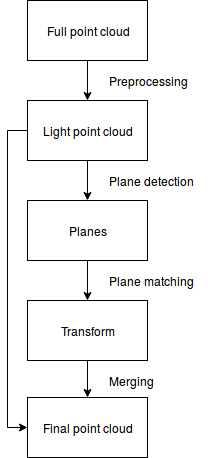
\includegraphics[scale=0.5]{images/pipeline_simple.png}
    \caption{Processing steps for one point cloud.}
    \label{fig:cut}
\end{figure}
